\documentclass{article}
\usepackage{amsmath}
\usepackage{amssymb}
\usepackage{graphicx}
\usepackage{hyperref}
\usepackage[version=4]{mhchem}

\title{Problem 9}
\date{}

\begin{document}
\maketitle

\section*{Problem}
(AMC) In the adjoining figure, \(C D\) is the diameter of a semi-circle with center \(O\). Point \(A\) lies on the extension of \(D C\) past \(C\); point \(E\) lies on the semi-circle, and \(B\) is the point of intersection (distinct from \(E\) ) of line segment \(A E\) with the semicircle. If length \(A B\) equals length \(O D\), and the measure of \(\angle E O D\) is \(45^{\circ}\), then the measure of \(\angle B A O\) is\\
(A) \(10^{\circ}\)\\
(B) \(15^{\circ}\)\\
(C) \(20^{\circ}\)\\
(D) \(25^{\circ}\)\\
(E) \(30^{\circ}\)

\section*{Solution}
(B).\\
Connect \(O B\).\\
Since \(A B=O D=O B, \angle B A O=\angle B O A=y\).\\
Since \(\angle O B E\) is the exterior angle of \(\triangle A B O\), \(\angle O B E=2 y\).\\
Since \(O B=O E, \angle O B E=\angle O E B=2 y\).\\
Since \(\angle E O D\) is the exterior angle of \(\triangle A O E\),\\
\centering
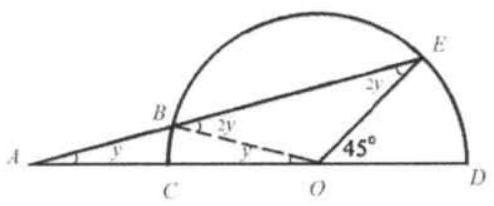
\includegraphics[width=\textwidth]{images/159(2).jpg}\\
\(\angle E O D=2 y+y=3 y=45^{\circ}\).\\
\(y=15^{\circ}\).\\

\end{document}
